%!TEX root = ../main.tex
\chapter{Introduction}\label{ch:intro}

This report supports the associated master project for handwriting recognition in difficult business documents. It presents a detailed view of our research and describes the steps we took to implement a working system. In addition, it grounds the problem in the existing body of work and motivates our choices with respect to various obstacles.

The rest of the chapter presents the context of the task, including motivation, challenges, related work and the goals we have set. \Autoref{ch:detection} is dedicated to the text detection part, presenting two different architectures and several experiments. Then, \autoref{ch:transcription} presents the second, and more difficult problem of text transcription from the images. We give a detailed analysis of important factors, which is supported by another large series of investigations. Each of the two parts also has a section dedicated to evaluation of the results. Finally, we conclude with \autoref{ch:conclusions} by listing our achievements and future work.


\section{Motivation}
At AXA, approximately 200\,000 accident statements need to be processed every year. But before any of these can be underwritten, human operators need to confirm them with the clients and register them in a database by transcribing the important information. This is a very slow process that requires precious human time before any value can be created for either the client or the company. As such, it would be of great help if the labour-intensive part could be automated and people could focus on more important tasks.

Given that a digital copy of all past statements has been kept for archival purposes, the task is to utilise them for speeding up the processing of future ones. This is, without a doubt, a very broad requirement, especially since in general only a few fields on the form are crucial for the company, while the others are needed mostly for the details of the accident and have to be confirmed by phone with the client. However, keeping the task broad adds a useful challenge to the project by ensuring a larger scope and utility.

\section{Challenges}\label{sec:challenges}
% Say we are only concerned with *offline* recognition. use this to explain : % http://ieeexplore.ieee.org/stamp/stamp.jsp?tp=&arnumber=367882 and this R. Plamondon and S. N. Srihari.  On-line and off-line handwriting recognition: a comprehensive survey. IEEE Transactions on Pattern Analysis and Machine Intelligence , 2000

Given the loose requirements above, the scope of the project was set to be an exploratory one, to investigate the capabilities of the state of the art approaches in \emph{offline} text recognition, and to adapt them to our needs. We want to extract as much data as possible from the statements, while keeping a general and flexible approach that can be applied to different formats and, later on, to different types of documents. Offline recognition means we have only the final image of the text, as opposed to the online case where the path of the pen is sampled during writing. The offline version is notoriously more difficult since the time order of the path is lost.

During phase zero of the project, we carried out extensive data screening in order to understand the format of the accident statements and the challenges it poses. In this section we expose the main take-aways of this process, along with the identified constraints and how they dictate the path we need to follow.

%----------------------------------------------------------------------------------------

\subsection{Format}
	\urldef{\transkribus}\url{https://transkribus.eu/Transkribus/}
	\begin{figure}
		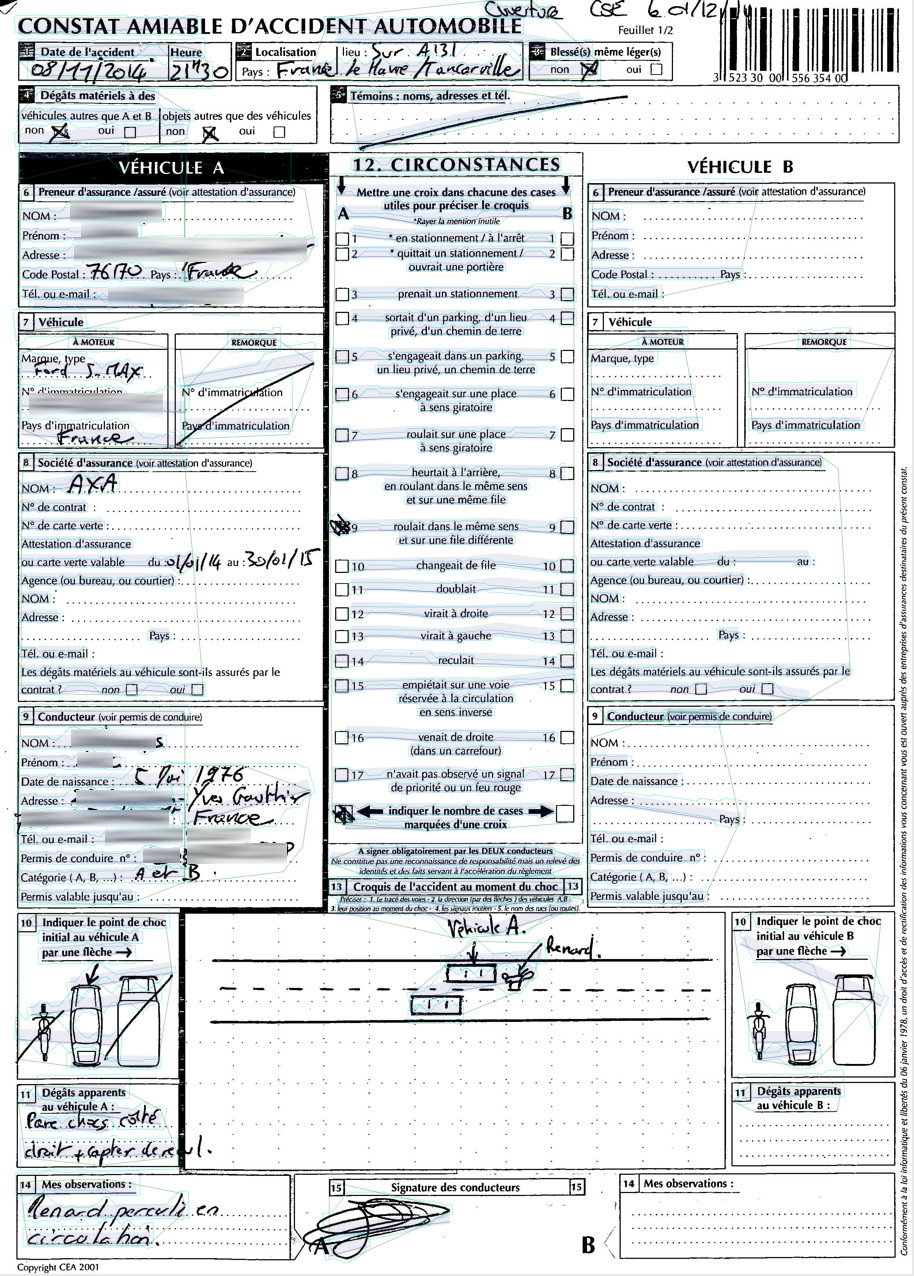
\includegraphics[height=.9\textheight]{transkribus_blur}
		\caption[Transkribus page segmentation]{The highlighted boxes correspond to locations of text according to a standard tool for handwriting transcription. Note we have blurred some lines \emph{after} the detection to preserve anonymity.}\label{fig:standard_tools}
	\end{figure}
	Standard OCR and HWR tools (Tesseract, Transkribus\footnote{\transkribus}) do not work well on our problem (\autoref{fig:standard_tools}). We believe this is due to:

	\begin{description}
		\item[the irregular format] Both tools expect text to be in a well structured format: words grouped into lines, lines grouped into paragraphs that span either the full page or are grouped into columns. In general, they can deal with local irregularities, such as a picture or quote which interrupts the normal flow. However, none of these groupings appear in our documents.

		\item[a mix of styles] OCR tools expect to have only printed text and treat everything else as an image. Conversely, HWR tools expect to have only handwritten text, and treat everything else as background or noise. As such, the heuristics for text line detection and segmentation fail on both types of tools, due to the presence of the other type of text.

		\item[Constraints] Such tools usually assume various constraints about the text. For example Tesseract needs to know the language of the text in advance. This does not apply in our case, as most of the text is unconstrained: dates, numbers, addresses, names. These do now follow the structure of a language.
	\end{description}

	We can note, however, that the statements \emph{do} subscribe to a certain, albeit non-standard, format. Text entry zones are indicated by a line, preceded with the name of the field in the language of the country. These are logically grouped into categories such as Policyholder, Vehicle, Insurance company etc., and each category has a unique identifying number (in the upper left corner). The personal information of the two persons is separated on the left and right sides by a set of check-boxes which describe the accident conditions.

	The logical grouping of fields into categories, along with their associated ID have become almost standard across the European Union and even neighbouring countries. However, only the \emph{content structure} seems consistent, whereas the actual placement of fields on the page can be significantly different.


%----------------------------------------------------------------------------------------


\subsection{Quality}

	During the acquisition and digitisation process many factors contribute to the final quality of the scan. First, we may get a ``$n$-th'' copy of the original, each stage degrading the signal and introducing noise. In some cases, even the ``original'' is, in fact, a carbon paper copy. In some other cases, the support paper is thin enough that data from the verso is visible on the scan. Also, probably for legacy reasons of disk space efficiency, most of the image information is discarded and only a 1-bit depth version is kept (binary image). This prevents colour-based segmentation of the image.

	However, the biggest source of inaccuracies and inconsistencies is the relatively unconstrained format of the statements. The persons completing such an accident statement are free to:
	\begin{description}
		\item[choose the format of the input data] For example \texttt{27 Apr 94} and \texttt{04/22/1994} are both valid entries for a date. This lack of rigor is especially problematic for addresses.

		\item[use the available space to their pleasing] In many cases, the given bounds are not respected and resulting text exceeds them horizontally or vertically. Often enough, people also ignore the labels and write in non-standard places.

		\item[use their natural handwriting] \label{itm:natural_handwriting} This introduces a great degree of variability for text entries, as well as ambiguity. As seen in \autoref{fig:context}, one person's \texttt{1} can resemble another person's \texttt{A}, and only the context helps us infer the word.

		\item[use any vocabulary they consider suitable] This often results in non-standard abbreviations or partial words (\autoref{fig:abbrev}).
	\end{description}

	\begin{figure}
		\begin{subfigure}[b]{.5\linewidth}
			\centering
			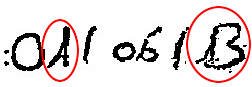
\includegraphics[width=.75\linewidth]{context}\\
			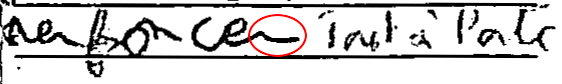
\includegraphics[width=.75\linewidth]{context2}
			\caption{}\label{fig:context}
		\end{subfigure}
		\begin{subfigure}[b]{.48\linewidth}
			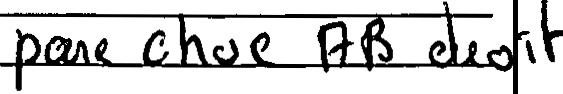
\includegraphics{abbrev}
			\caption{}\label{fig:abbrev}
		\end{subfigure}
		\caption[Ambiguity in handwriting]{In \subref{fig:context}, the highlighted glyphs are highly ambiguous either because they look like something else (top image: \(\mathtt{1} \rightarrow \mathtt{A}, \mathtt{13} \rightarrow \mathtt{B} \)) or because they look like no discernible character on their own (bottom image).\\
		In \subref{fig:abbrev}, we see people use custom abbreviations (``AB'') and write beyond the indicated box}
	\end{figure}


%========================================================================================


\section{Related work}\label{sec:related_work}
	Handwriting recognition is among the oldest and most common problems of machine learning. In fact, these days the recognition of handwritten digits has become the \textit{Hello world} equivalent of machine learning. For small examples like the MNIST challenge it works very well, to the degree that it can be considered a solved problem. However, the general scope of text detection and recognition, especially of handwritten type, is still an open research problem. In the past years many approaches have focused on the sister challenge, \emph{Optical Character Recognition} (OCR), because it can deliver more value to businesses while being easier to solve due to less variation in style.

	In what follows, we will list related work in this vast field, trying to summarise a few different approaches. A complete literature review is beyond the scope of this project. For each sub-problem, detection or transcription, we will try to distinguish between \emph{classical} techniques which employ hand-crafted features, and the \emph{modern} ones, which make use of neural networks for finding the best features of text.

	%----------------------------------------------------------------------------------------

	\subsection{Transcription}\label{sec:related_transcription}
		Early works for text recognition focused on simply classifying individual characters. \Citet{leCun_MNIST} presented a robust system for handwritten digit classification using Convolutional Neural Networks (CNNs). Their effectiveness has been proven over and over again, especially with the work of \citet{ciresan} who were the first to achieve near human performance on this task, while also improving the state of the art of the time on many image classification tasks.

		In order to deal with cursive writing, where character segmentation is more difficult, other works expanded the digit classification approach to words. For example, \citet{sharma2015adapting} adapt a pre-trained CNN to distinguish among classes of word images. This method requires fixed size input image and cannot deal with out-of-vocabulary words. \Citet{jaderberg2014_unconstrained} use an ensemble of character and n-gram CNNs to perform unconstrained recognition, but it only supports \emph{printed} words of length up to 23. \Citet{sudholt2016phocnet} provide a similar architecture which improves on these weaknesses by using Pyramidal Histogram of Characters (PHOC) as labels for the task of \emph{word spotting}.

		Another paradigm for dealing with cursive text is to use Recurrent Neural Networks (RNNs). This has gained momentum after the work of \citet{graves_LSTM} and \citet{graves_MDLSTM}, which excel at offline handwriting recognition. The former uses a heavy pre-processing pipeline for normalising the text image and extracts a collection of hand-crafted features for each column. These are then fed into a single-dimensional, bi-directional Long Short-Term Memory (LSTM) network \citep{LSTM_original}. The later provides a more general and robust system that works with raw pixel values and multiple languages at the same time by employing a multi-dimensional LSTM network. \Citet{MDLSTM_dropout} improves on the MD-LSTM architecture by carefully using dropout on the feed-forward connections.

		However, as \citet{MDLSTM_vs_CNN} notes, the MD-LSTM architecture has a significant computational cost and extracts features similar to the convolutional ones. Therefore, they propose a mix algorithm which reduces the input image into a series of convolutional features and predicts text using a 1-D LSTM network. \Citet{CRNN} use almost the same architecture for transcribing text in natural images.

	%----------------------------------------------------------------------------------------

	\subsection{Detection}\label{sec:related_detection}
		All the systems mentioned above focus solely on transcribing an already-segmented piece of text which comes from a clean database. In the real world, however, it is necessary to first locate the text and only then we can transcribe it.

		In the context of document analysis and form processing, classic approaches generally use a bottom-up strategy \citep{bottom_up}. After a binarisation step, foreground pixels are grouped into connected components. A filtering step based on blob's size is then applied in order to remove noise. Printed characters are separated from handwritten ones via profile projection matching \citep{profile_matching,moysset2014a2ia} or template matching \citep{template_matching}. Characters are grouped into words and text lines based on spatial proximity together with a Markov Random Field that models the dependency of neighbouring segments \citep{detection_mrf,detection_mrf2}. Alternatively, \citet{top_down} propose a top-down segmentation algorithm, but this is more suited for documents which present a well-formed Manhattan structure.

		Since \citet{ciresan} proved the high effectiveness of CNNs not only for text recognition, but also for a wide range of image classification tasks, they have been used to achieve high performance also in object detection. Two different meta-architectures dominate the field: ROI-based and direct methods.

		The first one relies on object candidates. The first work \citep{fast_rcnn} extracts them with classic region proposal algorithms and classifies them using a CNN in a predefined number of classes. The method is relatively time-consuming, owing to the large number of proposals that is needed for a high recall. \Citet{faster_rcnn} introduce a region proposal network (RPN) which achieves a good recall rate with far fewer proposals. This consists of a fully CNN that shares weights with the classifier, thus allowing it to be trained end-to-end. The shared computation also provides detection speed which is up to an order of magnitude faster than the previous implementation, hence the name \FRCNN{}. Slight modifications to this architecture are presented by \citet{deeptext} who adapt it for text detection by further reducing the number of proposals and applying multi-level ROI-pooling, along with a heuristic for Non-Maximum Suppression of overlapping boxes. \Citet{jaderberg} also present an architecture based on word-level region proposals. These are filtered with random forests and regressed with a CNN to be centred on the word. Finally, \citet{ctpn} note that text differs significantly from general objects since it can be arbitrarily long. Therefore, previous approaches which rely on a set of anchors with fixed aspect ratios do not scale well to this problem. Their solution extends the \FRCNN{} architecture by making the RPN output fine-scale proposals which are grouped into a bounding box by an LSTM network (see \autoref{sec:ctpn} for details).

		The second meta-architecture poses detection as a regression problem and passes the input image only once through a CNN. For example, \citet{ssd} predict class probability and offsets from a default bounding box at each location in the feature map, on multiple levels. Since they still use a set of anchors with a limited choice of aspect ratios, it fails to recognise long texts. \Citet{textboxes} fix this problem by using default boxes with large aspect ratios plus irregular $1 \times 5$ convolutional layers.

		The text-specialised methods above perform \emph{bounding box} detection at word or sentence level. Alternatively, \citet{moysset_whereToStart} detect only the height and the left start of a text line by using an architecture that interleaves convolutional and MD-LSTM layers. Then they delegate the task of finding the end of the line to the text recognition system.

	%----------------------------------------------------------------------------------------

	\subsection{End-to-end}\label{sec:related_e2e}
		In the very recent years, a new class of approaches emerged: \emph{end-to-end} architectures. These try to locate and transcribe text in a single pass, with errors from the transcription propagated back to the detection part. \Citet{attention_french} do so by coupling the convolutional feature maps with a two-dimensional attention model which they pass through an LSTM. In this way, the model can jointly learn where to look at each time step, and how to transcribe that information. However, this system can not identify the location of text in the image as a bounding box, only as a sparse attention map. \Citet{stn_ocr} overcome this limitation by using a spatial transformer network \citep{stn} for detection coupled with a ResNet-CNN for recognition. They acknowledge the system is difficult to train, requiring careful curriculum learning. Finally, we note that both of these approaches operate on printed text so they may not work well for handwriting. This is especially important for the latter one, as the recognition CNN processes independent regions of the image, thus relying on separation between characters.



%========================================================================================


\section{Objectives}

	Given the constraints imposed by our data and the weaknesses of classical approaches for HWR, we realise that our task is to find a robust way of identifying and transcribing handwritten text outside of a text context, which is also known as recognition of \emph{text in the wild}. To this end, we envision as end goal a system that can:
	\begin{enumerate}
	 	\item locate with good precision handwritten text in a document, and
	 	\item transcribe it, ideally with near human performance.
	\end{enumerate}
	We realise, however, that this may be an over optimistic goal, especially that we have no labelled data.

	It is important to note that matching text to its label in order to give \emph{structured} information is beyond the scope of the current work, partly because we view it as a less challenging task and partly because it is of no use without having the above system first.




